\section{QoSManager Framework}
\label{sect:qosmanager}
In this section, we describe the design and implementation of QoSManager. We first present
an overview of the design and then describe the important components in detail.

\subsection{Overview}

\begin{figure}[htb]
\centering
\includegraphics[width=0.5\textwidth]{arch}
\caption{QoSManager architecture}
\label{fig:architecture}
\end{figure}

QosManager is implemented as an application on top of a SDN controller. As depicted in \reffig{architecture},
the main components in QosManager are: 

\begin{itemize}
  \item \emph{Web Portal}: The web portal provides an interface for users to set QoS parameters for
    different types of traffic. In addition, users could also view the real time statistical information
    about the traffic flows from the web portal.
  \item \emph{Configuration Module}: The QoS policies are stored in a QoS configuration file in YAML~\cite{yaml} format. Configuration module mainly handles the configuration file and passes the QoS policies
    to the underlying three modules (traffic classification, forwarding and control, respectively).
  \item \emph{Traffic Classification Module}: The traffic classification module classifies the application
    type for each flow. It maintains a lookup table \emph{tc\_table} where the key \emph{id} is the hash value of a
    flow's five-tuple (e.g.,source IP address, destination IP address, protocol, source port and destination port).
    The value is the application type for the flow. Each table entry is also associated with a timestamp indicating
    when the flow starts. In the current implementation, the classification is performed by querying a statically
    defined database.
  \item \emph{Forwarding Module}: The forwarding module is responsible for making forwarding decisions (e.g.,
    to which port the packet should be sent). Currently, we implement a simple L2 switch. The more sophisticated
    forwarding module is discussed in \refsect{future}.
  \item \emph{Control Module}: The control module is the core of QosManger. It dynamically computes the
    assignments of flows to queues with appropriate sending rates based on the QoS policies, the global
    information about the flows in the network.
  \item \emph{Traffic Monitor Module}: The traffic monitor module monitors the traffic flows in the network
    and constantly reports the flow status information and the port status information to the web portal.
\end{itemize}

When the first packet of a flow arrives at a switch, it does not match any entries in the flow table(s), and
it is forwarded to the controller. The Ryu SDN controller receives a \textsf{PacketIn} event and passes the
packet to QoSManager. QosManager calls the traffic classification module to classify the application type for
the flow and stores the result with a timestamp in a lookup table \emph{tc\_table}. QoSManager then invokes
the forwarding module to make the forwarding decision. The forwarding module basically implements a simple L2
switch and maintains a \emph{mac\_to\_port} table. Subsequently, QoSManager calls the control module to compute
the assignments of flows to queues with appropriate rates. Based on the forwarding decision and the assignments,
QoSManager directs the controller to send \textsf{FlowMod} messages to the switch. In addition, when a flow is
removed from a switch, the controller will receive a \textsf{FlowRemove} event and pass the flow information to
QoSManager. QosManager then invokes the control module to recompute the assignments and send \textsf{FlowMod}
messages. Note that a flow added or removed may affect the assignments of multiple flows and thus multiple
\textsf{FlowMod} messages will be sent to the switch.\todo{Add outline for subsections} 

\subsection{QoS Policy}
\label{sect:qosPolicy}

An entry in a QoS policy configuration is defined as:

\begin{lstlisting}[basicstyle=\sffamily]
<application_type>:
  minimum: <integer> Kbps
  recommended: <integer> Kbps
  priority: <integer>
\end{lstlisting}

For each type of application (e.g., video, VoIP, gaming, P2P, etc.), users needs to configure 3 parameters. The \emph{priority}
parameter specifies the users' preference for the application. The higher the value is, the more important this type of
application is. We noticed that applications such as video streaming usually have different levels of QoS. Thus, we introduce two
parameters instead of one parameter to specify the requirement for an application. The \emph{minimum} parameter specifies
the minimum bandwidth the application requires. The \emph{recommended} parameter specifies the desired bandwidth for best
performance. For example, as shown in \reftable{qos_config}, the minimum bandwidth required by VoIP is 400Kbps and the recommended
bandwidth is 1.2Mpbs. The priority of VoIP, which is 10, is higher than any other types of services, so QoSManager will first try to
satisfy the QoS requirements for VoIP services.

\subsection{Control Module}

\begin{figure}[htb]
  \centering
  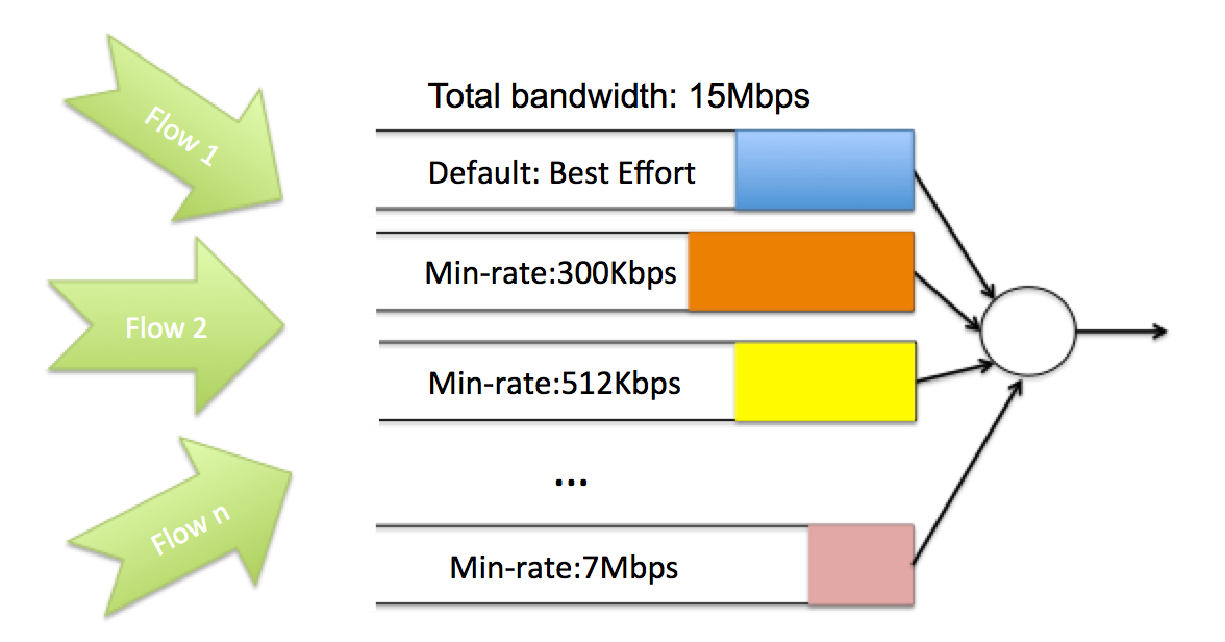
\includegraphics[width=0.5\textwidth]{assign_queue}
  \caption{QoSManager per-flow rate control.}
  \label{fig:assign_queue}
\end{figure}

The control module is the core of QoSManager. The goal of the control module is to assign an appropriate rate to each flow so that
the QoS of high priority applications can be effectively enforced. However, existing home routers do not support per-flow rate control,
and even the Open vSwitch (OVS) does not yet support per-flow QoS described in OpenFlow 1.3 specification~\cite{openflow13}. To overcome
this limitation, QosManager enables per-flow rate control by creating a list of queues with different sending rates at the ports of
the shared link \footnote{Here we assume that all the flows share a single link as shown in ~\reffig{setup}}. As shown in \reffig{assign_queue},
suppose the link capacity of the share link is \emph{C}, for each distinct bandwidth \emph{B} in the QoS policy configuration file,
we create $ N = \lfloor C / B \rfloor $ queues with minimal rate B and maximal rate C. In addition, we create a special queue $q_0$
only with maximal rate C. At runtime, QoSManager will assign each flow to a queue with an appropriate rate to control the rate of the
flow. Any flow that can not be guaranteed any level of QoS, it will be directly assigned to $q_0$.

To achieve the goal of the control module, we define the QoS utility function (\refsect{qosUF}) and propose a queue assignment
algorithm (\refsect{queueAssignAlgo}) to maximize the function under the limited link capacity.

\subsubsection{QoS Utility Function}
\label{sect:qosUF}
If the total bandwidth required by all the flows through a link exceeds the link capacity, it is obvious that the QoS requirements for
all the flows can not be fully satisfied, and we need to somehow prioritize the applications' traffic flows. In order to quantify the QoS
requirements satisfied, we assign a score to each flow. The score function for a flow \emph{f} is defined as:
\begin{equation}
\scalebox{0.9}{
  $score(f) =
    \begin{cases}
      priority       & \quad \text{if } bw(f) = \text{ recommended}\\
      0.5 \times priority & \quad \text{if } bw(f) = \text{ minimum}\\
      0              & \quad \text{if } \text{otherwise}\\
    \end{cases}$
}
\end{equation}

The score function basically says that if a flow can not be guaranteed any level of QoS, it gets 0 point. To distinguish between different
levels of QoS, we give full score to a flow if it is given recommended bandwidth and partial score to a flow if it is given minimum bandwidth.
We directly use priority as score. Therefore, higher priority application flow will get higher score if it is satisfied. Based on the score
function, the goal is to maximize the QoS utility function given a shared link with the capacity \emph{C}:

\begin{equation}
\begin{split}
  U_{QoS} = \sum_{i=1}^{n} score(f_i) \\ 
  \text{under } \sum_{i=1}^{n} bandwidth(f_i) \leq C
\end{split}
\end{equation}

It is clear that high priority application flows are more likely to be assigned their recommend bandwidth \emph{all the time}, and the QoS of low
priority flows may be sacrificed. Moreover, the bandwidth allocated to high priority application will not be affected by new low priority flows
going through the link. It is possible that the total score of some lower priority flows is greater than the score of a high priority flow, and
they cost less bandwidth. In that case, the bandwidth allocated to the high priority flow will be degraded. However, users can always tune the
priority at runtime to avoid this problem.

\subsubsection{Queue Assignment Algorithm}
\label{sect:queueAssignAlgo}

The optimization of the QoS utility function is very similar to the Knapsack problem~\cite{knapsack} which can be effectively solved by dynamic
programming. However, our problem differs form the canonical bounded knapsack problem in two ways. First, in our settings, an ``object" (flow) has
two ``values" (full and partial score) and two corresponding ``volumes" (recommended and minimal bandwidth). You can only choose one of them to put
into the ``knapsack" (shared link). Second, in order to avoid fluctuation, we want to keep a flow in the same queue as long as possible. That being
said, when new objects come, and we need to reorganize the knapsack, we want to keep as many old objects in the knapsack as possible. What's more,
since the knapsack is usually much larger than the smallest object, it is not memory efficient to use the dynamic programming. Instead, we use
depth-first search (\refalg{queueAssignAlgo}) to search for the optimal assignment.

\begin{algorithm}[htp]
  \SetAlgoLined
  \SetKwFunction{algo}{algo}\SetKwFunction{proc}{dfs}
  \SetKwFunction{Sort}{Sort}
  \SetKwInOut{Input}{input}
  \SetKwInOut{Output}{output}
  \SetKwProg{myalg}{Algorithm}{}{}
  \scriptsize
  \Input{A List $flowList$}
  \Output{A Map $assign$}
  
  $flowList$ $\leftarrow$ \Sort($flowList$, key='timestamp')\;
  $flowList$ $\leftarrow$ \Sort($flowList$, key='priority', reverse)\;
  $best\_score \leftarrow 0$ \;
  $N \leftarrow flowList.length$ \;
  $dfs(0, 0, 0, newList())$ \;
  \setcounter{AlgoLine}{0}
  \SetKwProg{myproc}{Procedure}{}{}
  \myproc{\proc{index, score, bw, temp\_assign}}{

  \uIf{ $index > N$ }{
    \uIf{$score > best\_score$}{
        $best\_score \leftarrow score $\;
        $assign \leftarrow temp\_assign$ \;
    }
  }
  $f = flowList[index] $\;
  \uIf{ $bw + f.recommend < C$ }{
    $temp\_assign.append(f.id, f.recommend) $\;
    $dfs(index+1, score+f.priority, bw+f.recommend, temp\_assign)$ \;
    $temp\_assign.removeLast()$ \;
  }
  \uIf{ $bw + f.minimum < C$ }{
    $temp\_assign.append(f.id, f.minimum)$ \;
    $dfs(index+1, score+f.priority*0.5, bw+f.recommend, temp\_assign)$ \;
    $temp\_assign.removeLast()$ \;
  }
  $dfs(index+1, score, bw, temp\_assign)$ \;
  }
  \caption{Queue Assignment Algorithm}
  \label{alg:queueAssignAlgo}
\end{algorithm} 


The algorithm takes a list \emph{flowList} and the shared link capacity \emph{C} as input. The \emph{flowList} merges the tc\_table and the
QoS policy configuration. We assume that all the flows in the \emph{flowList} are successfully classified by the traffic classification module.
If a flow can not be recognized by the traffic classification module, it will be directly assigned to $q_0$. The algorithm first sort the
\emph{flowList} by timestamp and then by priority. Suppose that the sorting algorithm is stable, and we will always pick the flows in a
``first come first serve" manner if there are multiple flows of the same application type. Then the algorithm invokes depth-first search procedure
to search for the optimal assignment.
